\section{THỰC NGHIỆM}

\subsection{Thiết kế Hợp đồng Cấu hình (Config Contract) và Sơ đồ Mạng PoC}

Để đảm bảo tính nhất quán và đồng bộ giữa các thành phần triển khai, dự án đã xây dựng một Hợp đồng Cấu hình chuẩn hóa làm nguồn sự thật duy nhất (Single Source of Truth) lưu giữ dưới tệp tin \texttt{CONFIG\_CONTRACT.yaml}. Hợp đồng này quy định chi tiết địa chỉ IP, cổng dịch vụ, phân đoạn VLAN và phiên bản phần mềm cho toàn bộ 5 máy chủ ảo trong hệ thống.

Mạng nội bộ được quy hoạch chi tiết trên dải IP \texttt{10.10.x.x} và phân chia thành 6 vùng mạng ảo (VLAN) logic độc lập nhằm triệt tiêu niềm tin ngầm định theo vị trí kết nối.

\begin{table}[H]
\centering
\caption{Bảng quy hoạch phân đoạn VLAN và địa chỉ IP hệ thống}
\label{tab:vlan_mapping}
\begin{tabular}{| c | p{3.2cm} | p{3.2cm} | p{2.8cm} | p{2.5cm} |}
\hline
\textbf{VLAN ID} & \textbf{Phân đoạn / Zone} & \textbf{Subnet IP} & \textbf{Gateway IP} & \textbf{Mục đích / Ghi chú} \\ \hline
10 & Client Zone & 10.10.10.0/24 & 10.10.10.1 & Thiết bị người dùng (DHCP) \\ \hline
20 & DMZ Zone & 10.10.20.0/24 & 10.10.20.1 & Pomerium Gateway (10.10.20.10) \\ \hline
30 & Security Zone & 10.10.30.0/24 & 10.10.30.1 & Keycloak IAM \& Wazuh Manager \\ \hline
40 & App Zone & 10.10.40.0/24 & 10.10.40.1 & Máy chủ ứng dụng OpenEMR \\ \hline
50 & DB Zone & 10.10.50.0/24 & 10.10.50.1 & Cơ sở dữ liệu MariaDB TDE \\ \hline
60 & Management Zone & 10.10.60.0/24 & 10.10.60.1 & Quản trị Proxmox VE (10.10.60.10) \\ \hline
\end{tabular}
\end{table}

\begin{figure}[H]
    \centering
    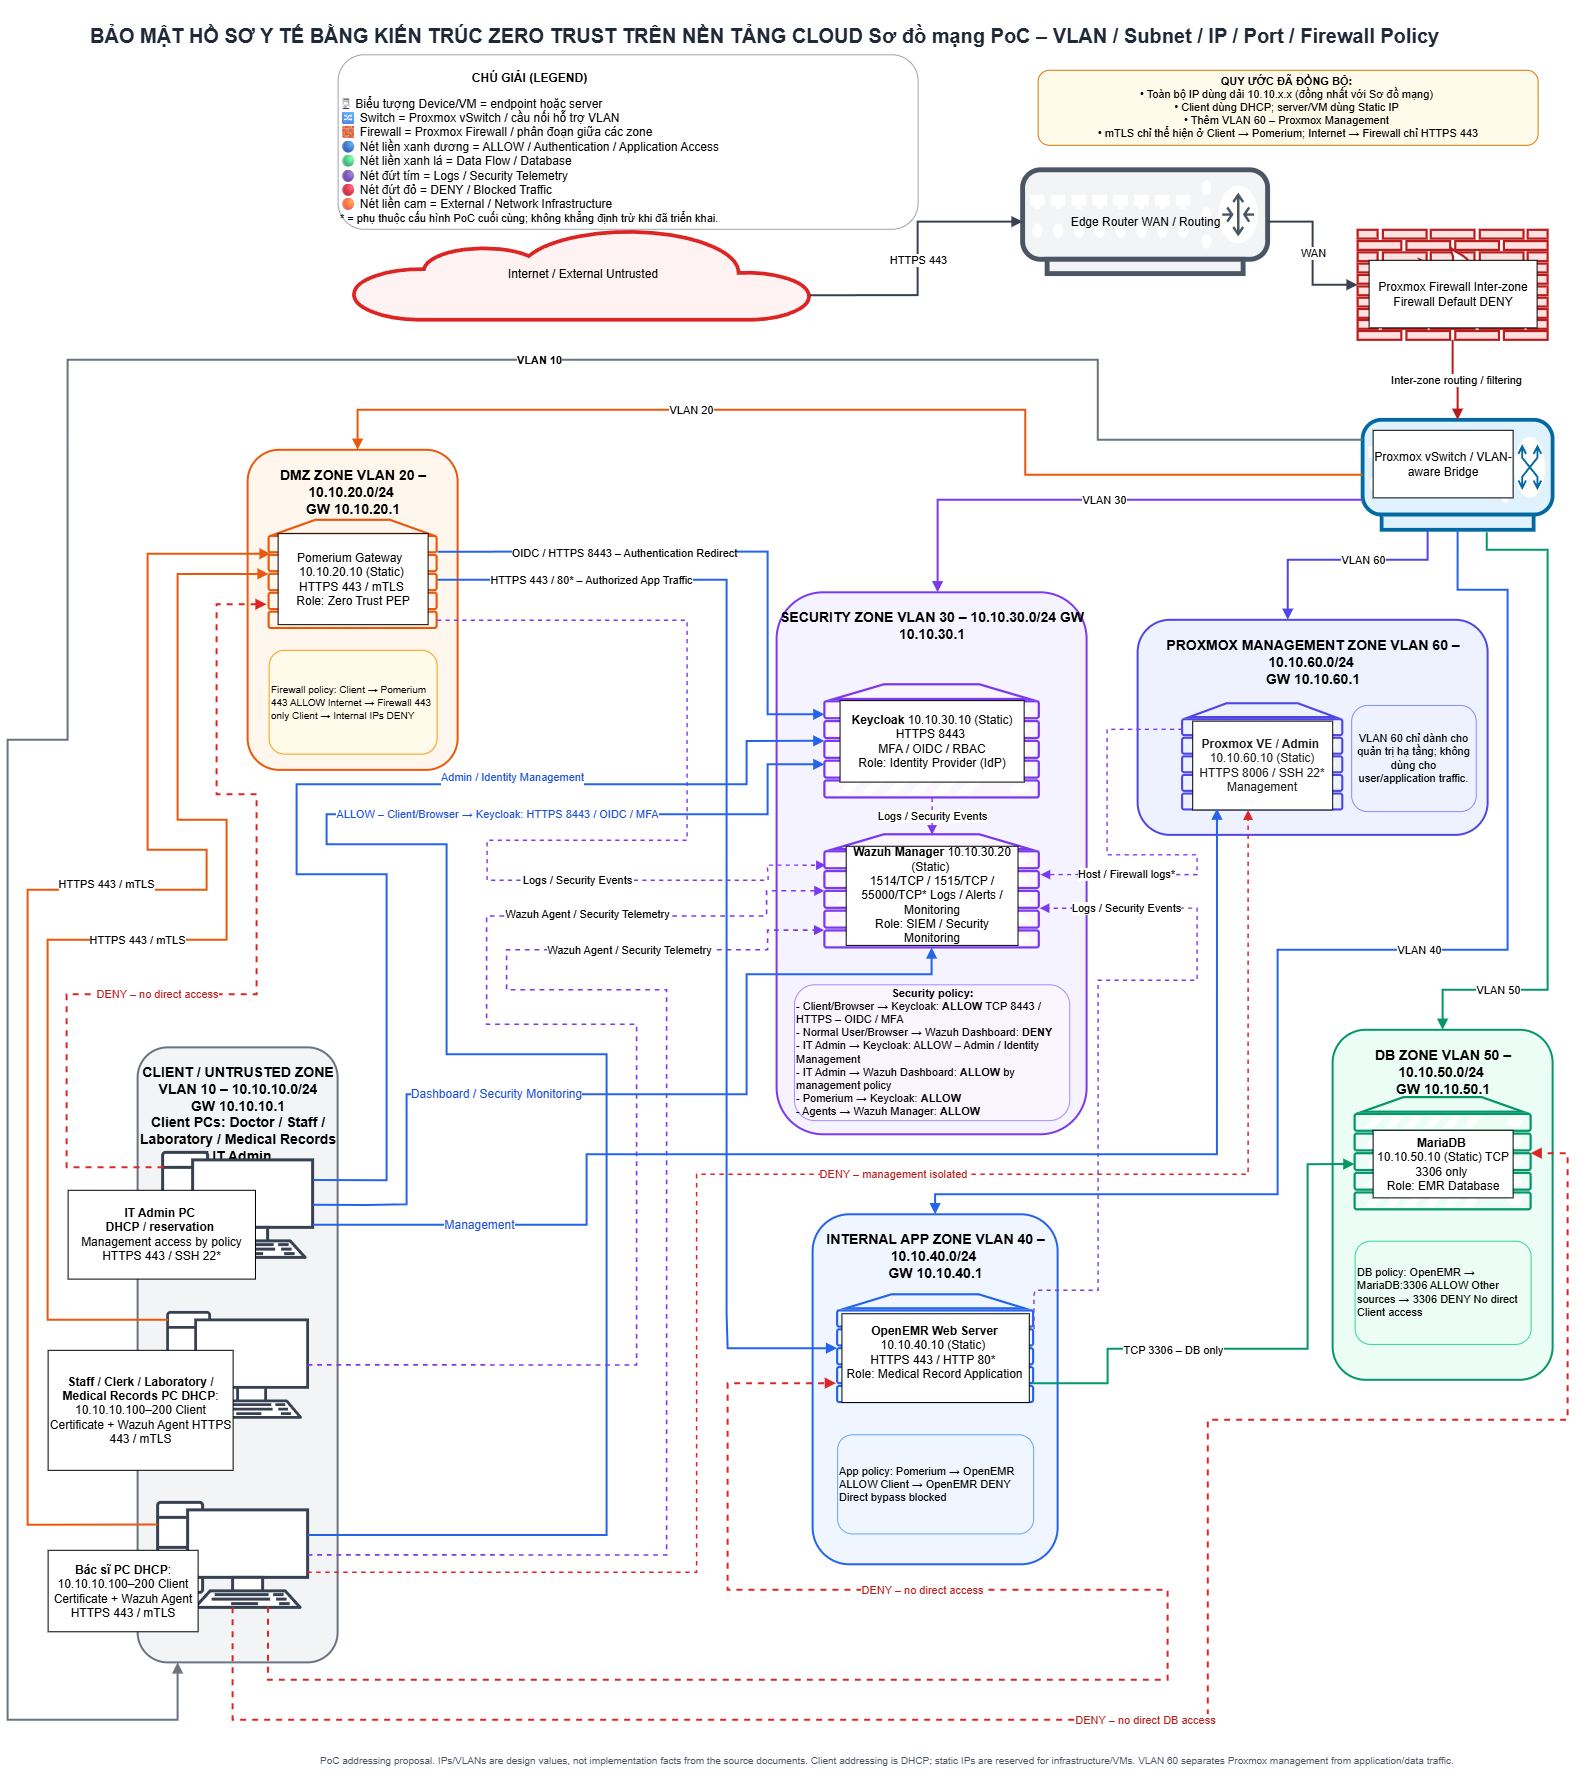
\includegraphics[width=0.95\textwidth]{image/zero_trust_medical_network_diagram_v3.drawio.png}
    \caption{Sơ đồ thiết kế phân đoạn mạng PoC Zero Trust bảo mật Hồ sơ Y tế Điện tử}
    \label{fig:network_diagram}
\end{figure}

\subsubsection{Giải thích Chi tiết Sơ đồ Thiết kế Mạng PoC (Hình 3.1)}

Sơ đồ thiết kế mạng PoC mô tả chi tiết hạ tầng mạng ảo hóa phân đoạn thành 6 vùng VLAN riêng biệt, quy định chặt chẽ các luồng dữ liệu được phép (ALLOW), luồng bị cấm (DENY) và luồng giám sát an ninh (Security Telemetry).

Phân đoạn 6 vùng VLAN cô lập: VLAN10 Client Zone (\texttt{10.10.10.0/\allowbreak 24}) chứa các thiết bị của người dùng (bác sĩ, kỹ thuật viên xét nghiệm, nhân viên y tế) kết nối; VLAN20 DMZ Zone (\texttt{10.10.20.0/\allowbreak 24}) đặt Pomerium Gateway tại IP \texttt{10.10.20.10}; VLAN30 Security Zone (\texttt{10.10.30.0/\allowbreak 24}) chứa Keycloak IAM (\texttt{10.10.30.10}) và Wazuh Manager (\texttt{10.10.30.20}); VLAN40 App Zone (\texttt{10.10.40.0/\allowbreak 24}) chứa máy chủ OpenEMR (\texttt{10.10.40.10}); VLAN50 DB Zone (\texttt{10.10.50.0/\allowbreak 24}) chứa MariaDB (\texttt{10.10.50.10}); và VLAN60 Management Zone (\texttt{10.10.60.0/\allowbreak 24}) dành riêng cho quản trị hypervisor Proxmox VE (\texttt{10.10.60.10}).

Phân tích các luồng mạng được cấp phép (ALLOW Traffic Paths): Người dùng truy cập từ VLAN10 gửi yêu cầu HTTPS 443 tới Pomerium Gateway tại VLAN20 kèm chứng chỉ mTLS. Pomerium gửi yêu cầu xác thực sang Keycloak tại VLAN30 qua OIDC HTTPS 8443. Khi người dùng hoàn thành xác thực và MFA, Pomerium chuyển tiếp lưu lượng được uỷ quyền (Authorized Traffic) sang OpenEMR tại VLAN40. Máy chủ OpenEMR kết nối truy vấn dữ liệu tới MariaDB tại VLAN50 duy nhất qua cổng TCP 3306.

Phân tích các luồng kết nối bị từ chối (DENY Traffic Paths - Nét đứt màu đỏ): Để triệt tiêu khả năng truy cập bypass cổng uỷ quyền và ngăn chặn di chuyển ngang (Lateral Movement), Tường lửa Proxmox Firewall thiết lập các quy tắc chặn tuyệt đối: Client không được phép truy cập trực tiếp vào OpenEMR (\texttt{Client -> OpenEMR: DENY}); Client tuyệt đối không có luồng kết nối tới MariaDB (\texttt{Client -> MariaDB: DENY}); và vùng Management cô lập hoàn toàn với dữ liệu ứng dụng.

Phân tích các luồng giám sát an ninh (Security Telemetry - Nét đứt màu tím): Tất cả các nút thành phần bao gồm thiết bị người dùng, Pomerium Gateway, Keycloak IAM, OpenEMR Web Server và Proxmox Hypervisor đều liên tục đẩy nhật ký sự kiện an ninh và telemetry về máy chủ trung tâm Wazuh Manager tại VLAN30 để theo dõi và phát cảnh báo thời gian thực.

\subsection{Triển khai Hạ tầng Ảo hóa Proxmox VE và 5 Máy chủ Ảo Skeleton}

Hệ thống ảo hóa được triển khai trên máy chủ Proxmox VE phiên bản 9.2-1 với hostname \texttt{pve01}. Cầu nối ảo mạng nội bộ \texttt{vmbr1} được cấu hình hỗ trợ \texttt{bridge-vlan-aware yes} với danh sách các VLAN ID từ 10 đến 60.

Năm máy chủ ảo Linux Debian skeleton đã được khởi tạo thành công trên Proxmox VE với cấu hình card mạng kép: một card kết nối mạng Internet tạm thời \texttt{vmbr0} để cập nhật gói tin và một card kết nối mạng nội bộ Zero Trust \texttt{vmbr1} được gán thẻ VLAN tương ứng.

\begin{table}[H]
\centering
\caption{Danh sách thông số chi tiết 5 máy chủ ảo Skeleton trên Proxmox VE}
\label{tab:vm_skeletons}
\begin{tabular}{| c | p{2.8cm} | c | c | c | c | p{3.2cm} |}
\hline
\textbf{VMID} & \textbf{Tên máy chủ ảo} & \textbf{VLAN} & \textbf{vCPU} & \textbf{RAM} & \textbf{Disk} & \textbf{Giao diện mạng nội bộ (net1)} \\ \hline
100 & emr-app01 & 40 & 2 & 2048MB & 32GB & vmbr1, tag=40 (VLAN40 App) \\ \hline
101 & zt-pomerium01 & 20 & 2 & 2048MB & 32GB & vmbr1, tag=20 (VLAN20 DMZ) \\ \hline
102 & zt-keycloak01 & 30 & 2 & 2048MB & 32GB & vmbr1, tag=30 (VLAN30 Security) \\ \hline
103 & zt-wazuh01 & 30 & 2 & 2048MB & 32GB & vmbr1, tag=30 (VLAN30 Security) \\ \hline
104 & emr-db01 & 50 & 2 & 2048MB & 32GB & vmbr1, tag=50 (VLAN50 DB) \\ \hline
\end{tabular}
\end{table}

\subsection{Cấu hình Hệ thống IAM Keycloak và Ma trận Phân quyền RBAC}

Máy chủ Keycloak được cài đặt trên VM102 và cấu hình Realm dành riêng cho hệ thống y tế mang tên \texttt{Hospital-Realm}.

Keycloak tiến hành định nghĩa các vai trò (Roles) cốt lõi phản ánh đúng cơ cấu tổ chức và ma trận phân quyền phòng khám bao gồm Doctor (Bác sĩ), Receptionist (Lễ tân), Lab (Kỹ thuật viên xét nghiệm), Records (Nhân viên quản lý hồ sơ), Medical Records Supervisor (Giám sát hồ sơ) và IT Admin (Quản trị viên CNTT).

Các tài khoản người dùng được tạo lập thử nghiệm và gán đúng vai trò tương ứng. Đồng thời, chính sách bảo mật bắt buộc cấu hình xác thực đa yếu tố (MFA) được kích hoạt. Khi đăng nhập lần đầu, người dùng bắt buộc phải sử dụng ứng dụng Google Authenticator trên điện thoại thông minh để quét mã QR và nhập mã OTP 6 chữ số.

\subsection{Cấu hình Cổng Uỷ quyền Pomerium và Tích hợp OIDC / mTLS}

Máy chủ Pomerium Gateway được cài đặt trên VM101, đóng vai trò trạm gác duy nhất tiếp nhận các kết nối HTTPS từ bên ngoài.

Pomerium được cấu hình tích hợp với Keycloak thông qua giao thức OpenID Connect (OIDC). Tệp tin cấu hình \url{config.yaml} của Pomerium khai báo \url{identity_provider_url} trỏ về Keycloak Realm và xác thực client secret.

Pomerium thiết lập các quy tắc phân luồng chính sách (Policy Routes): các yêu cầu định tuyến tới địa chỉ \url{https://emr.hospital.local} chỉ được cấp phép (Allow) nếu người dùng đã xác thực thành công qua Keycloak và sở hữu vai trò hợp lệ.

Để đảm bảo nhận diện thiết bị tin cậy, Pomerium được tích hợp chứng chỉ CA nội bộ được khởi tạo từ Easy-RSA. Pomerium bật tính năng xác thực hai chiều \url{downstream_client_ca}; các thiết bị người dùng nếu không được cài đặt chứng chỉ cá thể (.pfx/.crt) do CA nội bộ cấp sẽ bị từ chối kết nối ngay tại tầng giao vận TLS.

\subsection{Triển khai OpenEMR, MariaDB TDE và Giám sát Wazuh}

Ứng dụng OpenEMR được triển khai trên VM100 và được sử dụng làm hệ thống quản lý hồ sơ y tế trung tâm trong mô hình PoC. Theo kiến trúc, OpenEMR sẽ kết nối tới cơ sở dữ liệu MariaDB trên VM104 thông qua mạng nội bộ giữa VLAN40 và VLAN50 

Trên OpenEMR, nhóm xây dựng các vai trò nghiệp vụ gồm Lễ tân (\texttt{receptionist}), Bác sĩ (\texttt{doctor}), Kỹ thuật viên xét nghiệm (\texttt{lab}), Nhân viên quản lý hồ sơ (\texttt{records}), Giám sát hồ sơ (\texttt{medicalrecordssupervisor}) và Quản trị viên CNTT (\texttt{itadmin}). Tài khoản \texttt{admin} được sử dụng cho mục đích cấu hình và quản trị hệ thống ở mức cao nhất, không được xem là một actor nghiệp vụ trong ma trận phân quyền.

Cơ chế ACL/GACL của OpenEMR được sử dụng để giới hạn các chức năng mà từng vai trò được phép thực hiện theo ma trận phân quyền đã xác định ở Chương 2. Lễ tân được giới hạn ở các chức năng tiếp nhận và thông tin hành chính; Bác sĩ thực hiện các nghiệp vụ khám bệnh, ghi chú lâm sàng, chẩn đoán và chỉ định xét nghiệm; Kỹ thuật viên xét nghiệm xử lý chỉ định và kết quả xét nghiệm; Nhân viên quản lý hồ sơ khai thác hồ sơ trong phạm vi được phân công; Quản trị viên CNTT thực hiện các chức năng quản trị kỹ thuật nhưng không mặc định có quyền truy cập nội dung hồ sơ bệnh án.

Đối với vai trò Bác sĩ, quyền cập nhật dữ liệu chuyên môn được giới hạn theo bệnh nhân và lượt khám thuộc phạm vi phụ trách. Bác sĩ được phép tạo hoặc cập nhật ghi chú lâm sàng, chẩn đoán và chỉ định xét nghiệm đối với lượt khám thuộc phạm vi được phân công. Khi xét nghiệm đã được thực hiện và có kết quả, nội dung chỉ định liên quan không được tiếp tục thay đổi nhằm bảo đảm tính nhất quán giữa chỉ định và kết quả xét nghiệm.

Đối với vai trò Kỹ thuật viên xét nghiệm, người dùng được phép tiếp nhận chỉ định, cập nhật trạng thái xử lý và nhập kết quả xét nghiệm trong phạm vi nghiệp vụ được giao. Kỹ thuật viên xét nghiệm không được chỉnh sửa chẩn đoán hoặc ghi chú lâm sàng của Bác sĩ. Sau khi kết quả xét nghiệm đã được xác nhận, kết quả không được tiếp tục chỉnh sửa.

Bên cạnh phân quyền theo vai trò, nhóm bổ sung cơ chế \textit{Medical Records Assignment} nhằm giới hạn phạm vi bệnh nhân mà Nhân viên quản lý hồ sơ được phép truy cập. Vai trò \texttt{medicalrecordssupervisor} chịu trách nhiệm thực hiện assign hoặc reassign bệnh nhân cho người dùng thuộc vai trò \texttt{records}. Khi Nhân viên quản lý hồ sơ truy cập một bệnh nhân, hệ thống kiểm tra thông tin phân công trước khi cho phép khai thác các khu vực hồ sơ được bảo vệ. Nhân viên quản lý hồ sơ không được tự assign hoặc reassign hồ sơ cho chính mình, trong khi quyền quản lý assignment của Medical Records Supervisor không đồng nghĩa với quyền truy cập hoặc chỉnh sửa dữ liệu chuyên môn của bệnh án.

Trên VM104, cơ sở dữ liệu MariaDB được cấu hình kích hoạt tính năng mã hóa dữ liệu lưu trữ Transparent Data Encryption (TDE) thông qua plugin \url{file_key_management}. Tệp tin chìa khóa mã hóa được lưu trữ bảo mật và cấp quyền truy cập hạn chế cho dịch vụ mysql.

Dịch vụ giám sát Wazuh Manager được thiết lập trên VM103. Wazuh Agent được cài đặt lên tất cả 5 máy chủ ảo và cấu hình kết nối về Manager qua cổng 1514/1515. Wazuh kích hoạt mô-đun File Integrity Monitoring (FIM) theo dõi trực tiếp các tệp tin cấu hình nhạy cảm như \url{/etc/pomerium/config.yaml}, \url{/etc/mysql/mariadb.conf.d/} và phát cảnh báo tức thì khi có sự thay đổi trái phép.

Tường lửa Proxmox Firewall được thiết lập quy tắc chặn toàn bộ (Drop All) các kết nối mạng trực tiếp từ phân đoạn VLAN10 (Client) tới VLAN40 (App) và VLAN50 (DB), buộc tất cả lưu lượng bắt buộc phải đi qua đại diện uỷ quyền Pomerium Gateway tại VLAN20.
